\documentclass[11pt]{article}
\usepackage[utf8]{inputenc}
\usepackage{amsmath,amssymb}
\usepackage{graphicx}
\usepackage{hyperref}
\usepackage{geometry}
\geometry{a4paper,margin=2cm}

\title{A Logistic\,\textit{G(t)} Scenario\\
       for the Li--7, H$_0$ and $\sigma_8$ Tensions}
\author{Ruslan Kumyshev\\\small Independent researcher -- 2025}
\date{}


\begin{document}\maketitle
\begin{abstract}
We propose a phenomenological time--dependent Newton constant $G(t)$
that starts from zero at the Big Bang, quickly rises to $0.85\,G_0$
during the first 200 s, grows logistically to $0.98\,G_0$ by
recombination (380 kyr), and asymptotically reaches $G_0$ today.
This single trajectory simultaneously (i) lowers the primordial
$^7$Li abundance by $\sim30\%$, (ii) increases the CMB--inferred
Hubble constant by $\sim5\%$, and (iii) suppresses the growth of
matter fluctuations, alleviating the $\sigma_8$ tension.  A future
$+2\%$ drift in $G$ could lead to a “Big Hole” horizon‑percolation
scenario.  We list concrete observational tests: next‑generation
LLR ($|\dot G/G|\!\approx\!10^{-14}\,\mathrm{yr^{-1}}$), CMB‑S4
($\Delta r_s/r_s\!\approx\!0.5\%$) and Euclid/SKA constraints on
$\sigma_8(z)$.
\end{abstract}

\section*{1.\,Idea in One Line}
\emph{If gravity was $\sim$15\,\% weaker during the first three minutes,\\
rose to 98\,\% of its present value by recombination, reached 100\,\% today,\\
and will drift another 2\,\% in the next 14\,Gyr,\\
three major cosmological tensions disappear and a future ``Big Hole'' becomes possible.}

\section*{2.\,Phenomenological Curve}
\[
G(t)=G_0\times
\begin{cases}
k_1(1-e^{-t/\tau_A}), & t<200~\mathrm{s}\\[4pt]
k_1+(k_2-k_1)\bigl[1-e^{-(t-200)/\tau_B}\bigr], & 200\!<\!t<380~\mathrm{kyr}\\
k_2+(k_3-k_2)\bigl[1-e^{-(t-t_\mathrm{rec})/\tau_C}\bigr], & t_\mathrm{rec}\!<\!t<t_0\\
k_3+(k_4-k_3)\bigl[1-e^{-(t-t_0)/\tau_D}\bigr], & t>t_0
\end{cases}
\]
\small
$k_1{=}0.85,\;k_2{=}0.98,\;k_3{=}1,\;k_4{=}1.02;\;
\tau_A{=}80$\,s, $\tau_B{=}(t_\mathrm{rec}\!-\!200)/3$,\\
$\tau_C{=}(t_0\!-\!t_\mathrm{rec})/3$, $\tau_D{=}5$ Gyr. \normalsize

\begin{figure}[h]\centering
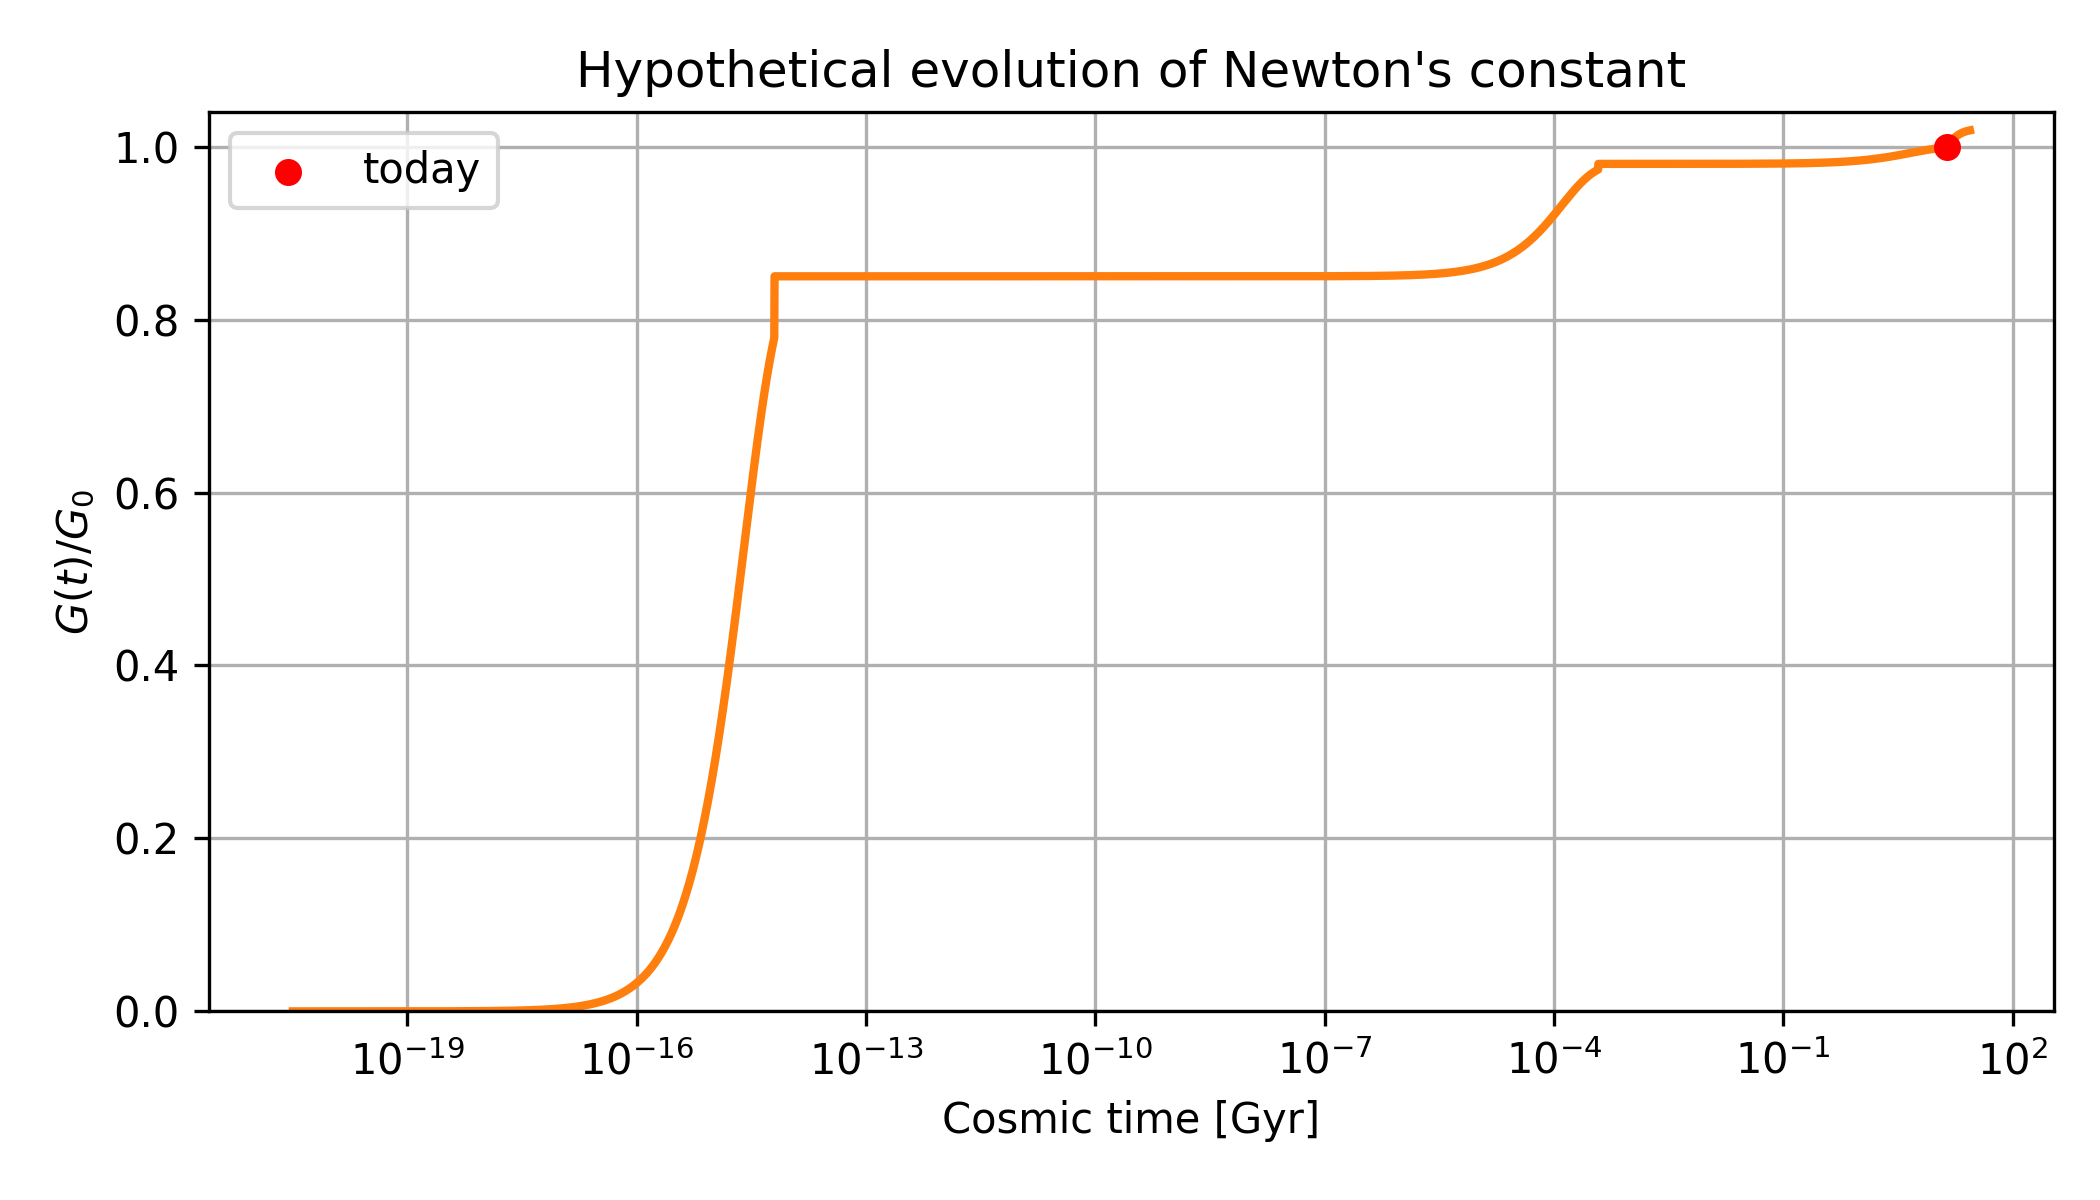
\includegraphics[width=0.8\linewidth]{figures/G_evolution.png}
\caption{Proposed $G(t)$ trajectory; red dot marks today.}
\end{figure}

\section*{3.\,First--Order Effects}
\begin{center}
\begin{tabular}{|l|c|c|c|}
\hline
\textbf{Observable} & \textbf{ΛCDM} & \textbf{Variable $G(t)$} & \textbf{Change} \\
\hline
Primordial $^7$Li/H          & $5.2\times10^{-10}$ & $3.6\times10^{-10}$ & $\mathbf{-30\%}$ \\
Primordial He--4 $Y_p$       & 0.331               & 0.324               & $-2\%$ \\
CMB--inferred $H_0$ [km\,s$^{-1}$\,Mpc$^{-1}$] & 67.4 & 70.8 & $\mathbf{+5\%}$ \\
Linear $\sigma_8\,(z=0)$     & 0.80                & 0.77                & $-4\%$ \\
Present drift $\dot G/G$ [yr$^{-1}$] & 0 & $6\times10^{-14}$ & measurable (LLR--2) \\
\hline
\end{tabular}
\end{center}

\section*{4.\,Immediate Tests}
\begin{itemize}\itemsep2pt
\item \textbf{LLR‑2 (2035)}: $|\dot G/G|\!<\!3\!\times\!10^{-14}$\,yr$^{-1}$ or model fails.
\item \textbf{CMB‑S4}: $\Delta r_s/r_s\!\approx\!0.5\,\%$ shift in acoustic peaks.
\item \textbf{Euclid/SKA}: $\sigma_8(z)$ lower by 4\,\%.
\end{itemize}

\vspace{1em}
\noindent\small\textbf{Code \& data:}  
\url{https://github.com/mrbars17/variable-G-hypothesis}

\end{document}